\section{Overview}\label{sec:overview}

\textbf{Fourier} is a four-input spectrum analyzer for VCV Rack 2. It shows
how a signal's amplitude is distributed across frequencies. Each input has
its own gain control and colored trace; the analysis and display controls
are shared by all four inputs. Fourier has no audio outputs: patch a signal
to it alongside your audio path to inspect the signal without changing it.

The analyzer uses a short-time Fourier transform (STFT), with selectable
window functions, FFT lengths, and intervals between analyses. Time and
frequency smoothing help reveal broad trends, while frequency bounds and
amplitude scales let you inspect a smaller part of the spectrum. A slope
control tilts the displayed amplitudes around $1\,\mathrm{kHz}$.

Fourier and Spectre belong to the Arhythmetic Units Fourier plugin.
Use Fourier to compare the current spectra of up to four signals, and
Spectre to follow one signal's spectrum over time. Both provide the same
window choices and smoothing controls, but their display axes, input-gain
defaults, and Run behavior differ as described below.

The module takes its name from Jean-Baptiste Joseph Fourier
(Fig.~\ref{fig:fourier-portrait}), whose work describes signals in terms of
simpler trigonometric functions.

\begin{figure}[!htp]
\centering
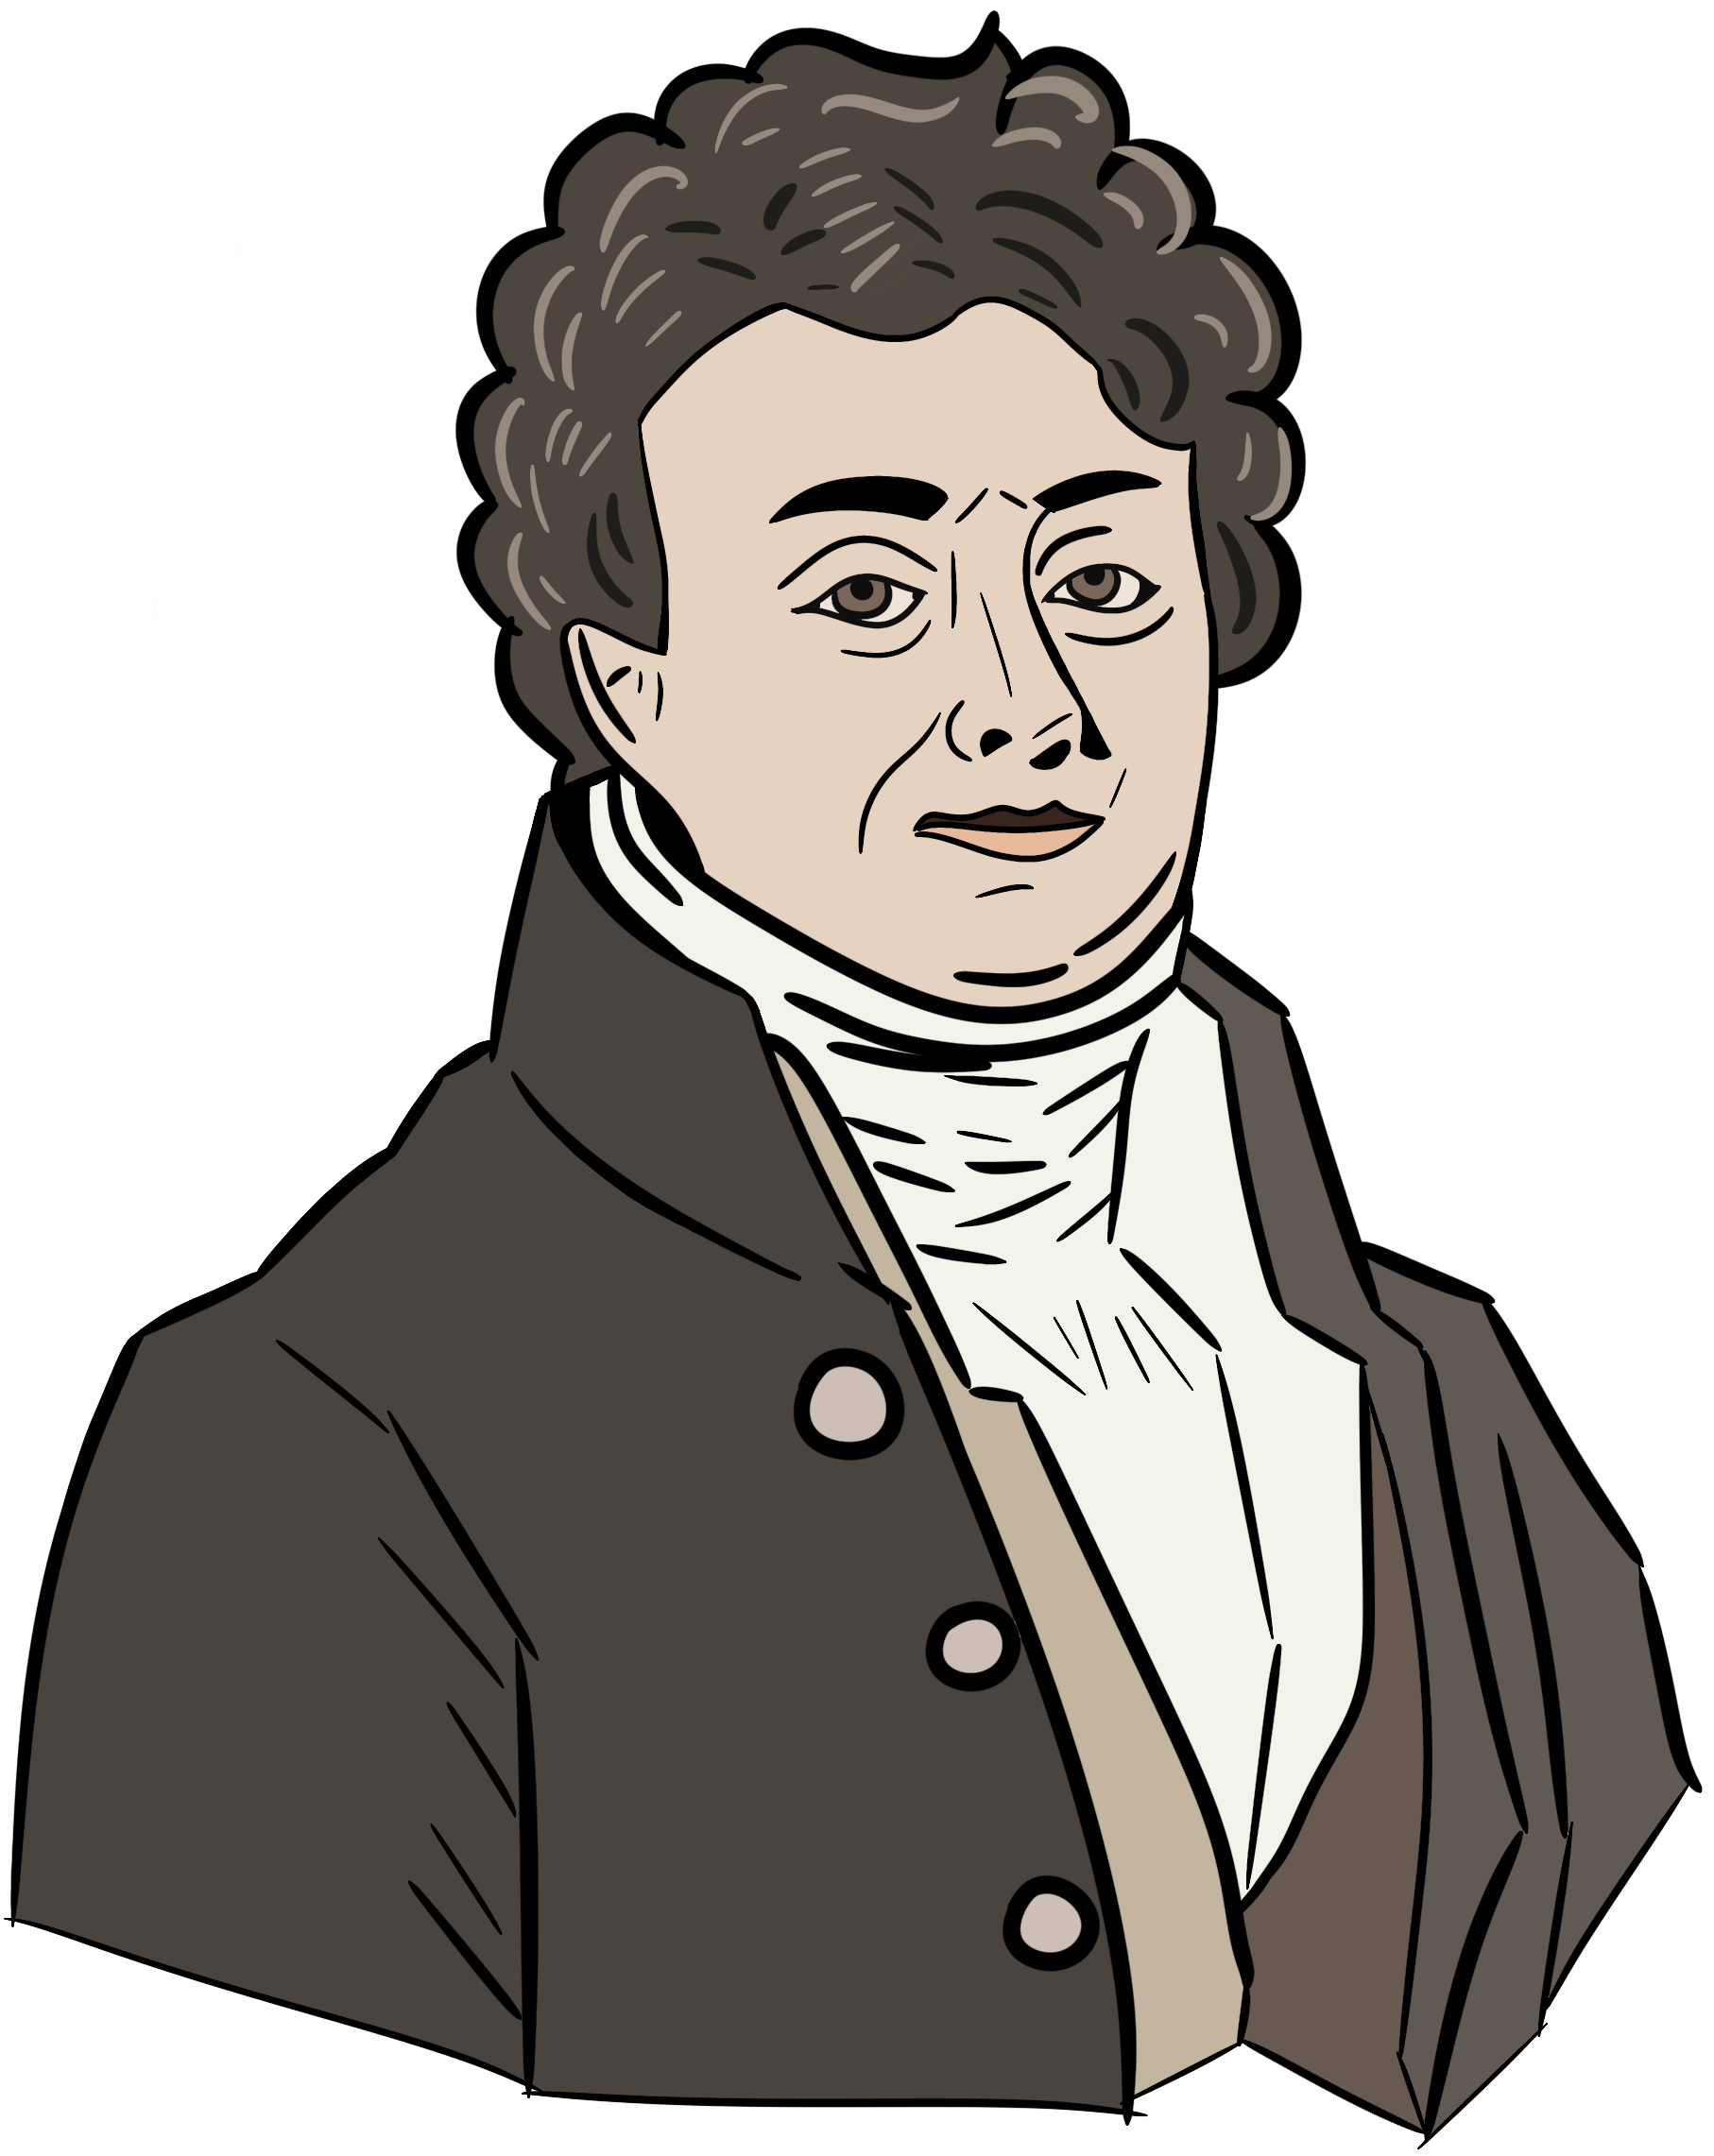
\includegraphics[width=0.38\textwidth]{img/FourierPortrait}
\caption{Jean-Baptiste Joseph Fourier (March 1768 -- May 1830).}
\label{fig:fourier-portrait}
\end{figure}
